\chapter{\fancyname{ReactMPST}: Front-End Session Type Web Development}
\label{chap:react}

In this chapter, we present \fancyname{ReactMPST},
our session type API generation strategy for browser-side endpoints
implemented using React \cite{React}.
We will refer to the FSM of the \trole{Client}
endpoint (\cref{fig:adderclientfsm})
from the \tprotocol{Adder} protocol 
throughout this chapter.

\begin{figure}[!b]
\centering
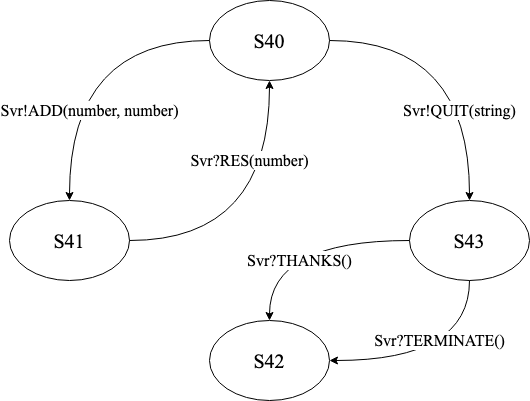
\includegraphics[width=0.55\textwidth]{AdderClientFSM}
\captionof{figure}{\trole{Client} Endpoint FSM
in \tprotocol{Adder} protocol}
\label{fig:adderclientfsm}
\end{figure}

\section{Challenges}
\label{section:reactchallenges}

Our goal with \reactcodegen is to
generate session type implementations for the web browser.
Integrating session types into user interfaces is inherently difficult --
assuming channel actions are bound to user interface events 
(i.e. clicking a button sends a message), how does one formalise
channel linearity? How do we guarantee that, if the button
triggers a send at some EFSM state, that it triggers not more than
one channel action, \textit{and} the user cannot trigger the action
at another EFSM state?

We recap how existing work 
(as discussed in \cref{subsection:sessiontypewebdev})
tackle browser-side session typing.
Fowler \cite{MVU2020} introduced the concept of model types to 
prevent
channel linearity violation in his proposal for
integrating session types with
GUI programming, but
it uses the Links web programming language \cite{LINKS} which
lacks compatibility with the ecosystem of JavaScript
libraries that one might use in front-end development as well.
The session type-safe web development framework presented
by King et al. \cite{PureScript2019} generates APIs for
a functional target language in PureScript, and relies on
the \textit{Concur UI} framework that constructs UIs sequentially.

As motivated in \cref{section:intro},
we find these proposals to come at the cost of
limiting developer productivity by adopting unconventional practices
that may require a learning curve.
Through our work, we aim to distil the key
concepts from \cite{MVU2020,LINKS,PureScript2019} 
that provide session type safety
for web-based GUI programming, and implement them using
mainstream front-end web development tools (specifically TypeScript
and React), to provide developers with an intuitive way to implement
browser-side endpoints that guarantee communication safety.
\section{Approach}
\label{section:reactapproach}

We motivate our approach from \cite{MVU2020} by extending
their work on \textit{multiple model types} motivated by the
\textit{Model-View-Update} architecture (MVU),
introduced in \cref{section:bgrelated}.
The concept of model types express type dependencies between these
components: a \emph{model type} uniquely defines a \textit{view function},
set of \textit{messages} and \textit{update function} -- rather than
producing a new model, the update function defines valid transitions to
other model types.

We leverage the correspondence between model types 
and states in the EFSM:
each state in the EFSM is a model type, the set of messages represent
the possible channel actions available at that state,
and the update function defines which successor state to transition to,
given the supported channel actions at this state.

We implement model types for the EFSM on top of the 
\emph{React.js} (React) framework developed by Facebook \cite{React}.
React is widely used in industry to create scalable single-page
web applications, so this makes our workflow beneficial in an
industrial context. 
The framework defines a way for data to flow
between UI elements, and empowers the UI to subscribe and
``react'' to data changes;
we introduce the framework in \cref{subsection:react}.
We aim to implement similar behaviour with respect to the EFSM:
the UI should react to EFSM state transitions,
so we can \textbf{statically} ensure that the
channel actions ``present'' on the browser at any given time
are those permitted by the current EFSM state.

When executing \reactcodegen to generate code
for the \trole{Client} endpoint specifying the
\texttt{browser} target, the developer obtains the following 
groups of files:

\begin{itemize}

\item 
\textbf{S[40-43].tsx\footnote{
The \filename{.tsx} file extension allows
for embedding \textit{JSX} \cite{JSX} elements inside the file.
JSX is a XML-like syntax extension to JavaScript
for elements and components.
}:}
Developer APIs for implementing EFSM states 
(\cref{section:reactefsm});

\begin{itemize}
\item
\textbf{EFSM.ts}, \textbf{Message.ts}, \textbf{Roles.ts:}
Utility types for EFSM encoding;
\end{itemize}

\item 
\textbf{Client.tsx:} 
Session runtime for executing the EFSM 
(\cref{section:reactruntime});

\begin{itemize}
\item
\textbf{Session.ts}, \textbf{Types.ts:}
Utility types for session runtime.
\end{itemize}

\end{itemize}

\subsection{The React Framework}
\label{subsection:react}

We introduce the key features of the framework
through illustrating a web-based counter in \cref{lst:counter}.
The browser shows a counter (initialised to zero) 
and an ``Increment'' button:
when the user clicks on the ``Increment'' button,
the count is incremented and the UI shows the updated count.

\begin{figure}[!h]
\begin{lstlisting}[language=javascript,tabsize=2]
type Props = { count: number };
class Count extends React.Component<Props>{
	render() { (*@\label{line:childrender}@*)
		return <strong>{this.props.count}</strong>; (*@\label{line:childprops}@*)
	}
}

type State = { count: number };
class App extends React.Component<{}, State>{
	constructor(props: {}) {
		super(props);
		this.state = { count: 0 }; (*@\label{line:parentstate}@*)
	}
	
	increment() { this.setState({ count: this.state.count + 1 }); (*@\label{line:parentsetstate}@*)
	
	render() { (*@\label{line:parentrender}@*)
		return (<div>
			<button onClick={this.increment.bind(this)}>
				Increment
			</button>
			<Count count={this.state.count} /> (*@\label{line:childcomponent}@*)
		</div>);	
	}
}
\end{lstlisting}
\captionof{lstlisting}{Simple Counter in React}
\label{lst:counter}
\end{figure}

\paragraph{Components}
A \textit{component} is a reusable UI element which
contains its own mark-up and logic.
Components implement a \texttt{render()} method which returns
a React element, the smallest building blocks of a React application.
This is analogue to the \textit{view} function in the MVU architecture.
React uses the \textit{JSX} syntax extension \cite{JSX}
to interpolate TypeScript logic 
(enclosed in curly braces)
within HTML mark-up: 
in \cref{line:childrender}, the \texttt{Count} component
evaluates the TypeScript expression 
\lstonelinejs{this.props.count} and renders it in bold on the web page.

Components can render other components, which give rise to
a tree of UI elements. \cref{line:parentrender} shows that our
\texttt{Count} component is rendered by 
the \texttt{App} component.

\paragraph{Uni-directional Data Flow}
User-defined components derive from the abstract base class
\texttt{React.Component<P, S>},
which is an abstract base class with generic type parameters
\texttt{<P, S>} for \textit{props} (short for properties) and 
\textit{state} respectively.

The \texttt{App} component maintains \texttt{count} in its
state (\cref{line:parentstate}). Clicking on the increment button
updates the state (\cref{line:parentsetstate}), which invokes
a re-render, so the UI ``reacts'' to state change.

Data flows from parent components down to their children,
in the form of props. 
The \texttt{App} component passes the \texttt{count}
from its state to the \texttt{Count} component 
(\cref{line:childcomponent}), which accesses it via
\lstonelinejs{this.props}. 
Because \texttt{App} is re-rendered when the count is incremented,
the \texttt{Count} child component will also be re-rendered
with updated props.

\paragraph{Virtual DOM (VDOM) and Reconciliation}
The \texttt{render()} methods give the developer a declarative API
to specify what should be rendered. React uses a 
\textit{virtual DOM} abstraction, where the tree of React elements
are rendered on the virtual DOM, and React internally
runs a \textit{reconciliation} algorithm to update the browser DOM
accordingly using minimal operations.

For example, the \texttt{<button>} will not be re-rendered
on the browser DOM on every counter increment as it does not
depend on the updated state.

\section{EFSM Encoding}
\label{section:nodeefsm}

We show the structure of the generated EFSM.ts file in
\cref{lst:nodeefsmfile}.
Note that the formal definition of the EFSM in 
\cref{section:scribbleefsm}
contains more than just states and the state transition function,
so we encode the additional information as well.
Each type of information is grouped into their own
\textit{namespace}, and are collectively exported in
the EFSM \textit{module} for the developer to use.

\begin{figure}
\begin{lstlisting}[language=javascript,tabsize=2,title=EFSM.ts]
// (*@\cref{subsection:nodeefsmroleslabelsmsg}@*)
export namespace Roles {...};
export namespace Labels {...};
export namespace Message {...};

// (*@\cref{subsection:nodeefsmhandlers}@*)
export namespace Handler {...};

// (*@\cref{subsection:nodeefsmimplementation}@*)
abstract class ISend {...};
abstract class IReceive {...};
abstract class ITerminal {...};
export namespace Implementation {...};

export type EfsmTransitionHandler =
	(implementation: Implementation.Type) => void;
export type MessageHandler = (message: any) => void;
\end{lstlisting}
\captionof{lstlisting}{Structure of Generated EFSM Encoding 
for Server Endpoint}
\label{lst:nodeefsmfile}
\end{figure}

\subsection{Roles, Labels, Messages}
\label{subsection:nodeefsmroleslabelsmsg}

We generate TypeScript constructs for these pieces of information
so they can be reused throughout the generated code, 
and in particular, the runtime.

\subparagraph{Roles}
The runtime needs to know the identifiers of participants involved
in the session, and who to send/receive from 
depending on the EFSM state.
We generate string enumerations, or \textit{enums}, for each 
participant in the protocol, \textit{excluding} the 
first person endpoint. 
The enum appropriately groups the collection
of participants involved and scales for multiparty sessions,
whilst making it simple to derive other types, e.g. a mapping from
participants (indexed by the enum) to WebSockets.

\subparagraph{Labels}
The runtime needs to decide which handler to invoke, based
on the label of the received message. Similarly, the developer needs
to provide handlers specifying their internal choice (e.g. which
message label to send) and how to handle external choice (e.g. 
how to handle received message with particular label).
For the same reason, we also generate string enums for message labels,
one enum per state. Enums are compatible with switch statements,
which can be used to dispatch messages to the correct handlers
in the runtime based on the message label. 
We give an example in \cref{lst:nodeefsmlabels}.

\begin{figure}[!ht]
\begin{lstlisting}[language=javascript,tabsize=2]
// Inside the Labels namespace...
export enum S51 { ADD = "ADD", QUIT = "QUIT", };
export enum S53 { RES = "RES", };
export enum S54 { THANKS = "THANKS", TERMINATE = "TERMINATE", };
\end{lstlisting}
\captionof{lstlisting}{Generated Label Enums for \trole{Svr} endpoint}
\label{lst:nodeefsmlabels}
\end{figure}

\subparagraph{Messages}
The handler APIs that we generate for developers
need to refer to the label identifier and payload type: 
we refer to this as the message structure, and encode this as a
Message Type. 
Each message is expressed as an interface with
properties for the label and payload.
These interfaces are grouped based on the EFSM state
they belong using \textit{union types}.
We illustrate this in \cref{lst:addersvrmsg}.
By expressing the payload type as a \textit{tuple}\footnote{
In TypeScript, a tuple is an array with fixed size
and known types for elements at each position.
},
we easily generalise our type definition to polyadic payloads.

\begin{figure}[!ht]
\begin{lstlisting}[language=javascript, tabsize=2]
// Inside the Message namespace...
export interface S54THANKS {
	label: Labels.S54.THANKS,
	payload: [string],
};
export interface S54TERMINATE {
	label: Labels.S54.TERMINATE,
	payload: [],
};

export type S54 = | S54THANKS | S54TERMINATE;
\end{lstlisting}
\captionof{lstlisting}{Generated Message Type Definition for State 54}
\label{lst:addersvrmsg}
\end{figure}

\subsection{Handler APIs}
\label{subsection:nodeefsmhandlers}

We collect the APIs that the developer needs to implement
under the \texttt{Handler} namespace. 
As a design choice, we \textit{do not} generate handlers for
terminal states, because the semantics of inactivity mean
there is nothing to handle.
We introduce the generated handlers for sending and receiving states.
These are non-terminal states that will involve the encoding of its
successor state. The reader will notice that, in the listings below,
the successor state is stated to be under the
\texttt{Implementation} namespace: we explain in 
\cref{subsection:nodeefsmimplementation}, but for now,
it is sufficient to acknowledge that those refer to the encoding
of the successor state.

\subparagraph{Send}
We model selections using a union type to
encapsulate the possible send actions, as shown in 
\cref{lst:addersvrsendhandler}.
Each send action is encoded as a tuple of
the label, the payload, and the successor state encoding.
We see some benefits from defining Message Types as interfaces:
TypeScript supports \textit{index type queries} to extract
named property types, so
\lstonelinejs{Message.S54THANKS['payload']} 
would resolve to \lstonelinejs{[string]},
based on the interface definition \cref{lst:addersvrmsg}.

\begin{figure}[!ht]
\begin{lstlisting}[language=javascript, tabsize=2]
// Inside the Handler namespace...
export type S54 = 
	| [Labels.S54.THANKS, Message.S54THANKS['payload'],
			Implementation.S52] 
	| [Labels.S54.TERMINATE, Message.S54TERMINATE['payload'], 
			Implementation.S52];
\end{lstlisting}
\captionof{lstlisting}{Generated Type for \trole{Svr} Send State
in \tprotocol{Adder} protocol}
\label{lst:addersvrsendhandler}
\end{figure}

We generalise deterministic send actions as a trivial \textit{selection}, 
as motivated from the theory (\cref{fig:globaltypes}),
so the encoding for State 53 in the \trole{Svr} FSM would be
the union of a single tuple.

\subparagraph{Receive}
We model branching using an interface to 
enumerate the possible branches, as shown in
\cref{lst:addersvrreceivehandler}.
As with send states,
we generalise deterministic receive actions as a trivial \textit{branch},
which would be an interface with one property. 

\begin{figure}[!ht]
\begin{lstlisting}[language=javascript,tabsize=2]
// Inside the Handler namespace...
export type S51 = {
	[Labels.S51.ADD]: (...payload: Message.S51ADD['payload']) =>
		Implementation.S53,
	[Labels.S51.QUIT]: (...payload: Message.S51QUIT['payload']) => 
		Implementation.S54,
}
\end{lstlisting}
\captionof{lstlisting}{Generated Type for \trole{Svr} Receive State
in \tprotocol{Adder} protocol}
\label{lst:addersvrreceivehandler}
\end{figure}

The interface properties are defined by the 
labels of the permitted receive actions:
the square-bracket notation means that the property name
is derived from the value of the enclosing variable,
so \lstonelinejs{[Labels.S51.ADD]} resolves to the
\lstonelinejs{'ADD'} string. 

The interface values are functions parameterised by
the message payload, and must return the successor state encoding.
We see another benefit of defining the payload in Message Types
as a tuple: we can define the receive handler parameter
using the \textit{spread syntax}, which allows the tuple
expression to be expanded into a list of function arguments. 
More concretely, as shown in \cref{lst:nodeefsmspread},
it allows the developer to pattern match on the
individual payload values (\cref{line:yesspread}) 
rather than defining their function to expect a tuple 
and manually destructing it (\cref{line:nospread}),
so the former is more intuitive.

\begin{figure}[!ht]
\begin{lstlisting}[language=javascript,tabsize=2]
const withSpread = (x: number, y: number) => {...} (*@\label{line:yesspread}@*)
const withoutSpread = (payload: [number, number]) => {...} (*@\label{line:nospread}@*)

const handler1: Handler.S51 = { ADD: withSpread		, ... };	// OK
const handler2: Handler.S51 = { ADD: withoutSpread, ... };	// OK
\end{lstlisting}
\captionof{lstlisting}{Example Handler Signature 
Compatible with Spread Syntax}
\label{lst:nodeefsmspread}
\end{figure}

\subsection{Wrapping Handlers in ``Implementations''}
\label{subsection:nodeefsmimplementation}

The behaviour of the runtime is dependent on the current state,
so it needs a way to distinguish between
all the different states -- one can think of this as implementing
the state transition function from the theory, which is analogue to 
overloading a \texttt{next()} method for each state.
Due to limitations in the TypeScript language, this would have to
be some sort of switch statement, with the \texttt{next()}
method parameterised by some base type assignable to all states.
Currently, the state is only determined by the handler
to be implemented by the developer, so the switch statement
and base type would have to be defined on the handler APIs.

Unfortunately, this is not practical. 
Handlers for send states are union types and
handlers for receive states are interfaces,
both of which are not supported 
by the \lstonelinejs{instanceof}
operator.

\subsubsection{Distinguishing Handlers using Conditional Types}

We attempt to address this by defining an enum of state identifiers
for each type of state (i.e. an enum for send states, 
an enum for receive states)
upon which to execute the EFSM, which solves the switch statement
problem.
Now, we are left with defining a mapping between the 
state identifier enum to the handler type. This construct would be
analogue to \textit{dependent types}, which again, is not a feature
of the TypeScript type system.

We try to define type dependencies using
\textit{conditional types} in TypeScript.
A conditional types is a type-level expression
\begin{lstlisting}[language=javascript,numbers=none]
T extends U ? X : Y;
\end{lstlisting}
which reads, \textit{if \texttt{T} is assignable to \texttt{U},
then the type is \texttt{X}; otherwise, the type is \texttt{Y}}.

Combined with \textit{generic constraints}\footnote{
\lstonelinejs{<T extends U>} defines a generic type \texttt{T}
and enforces that it must be a type assignable to \texttt{U}.
},
we can approximate the dependency between the state identifier
enum and the generated handler API using something
similar to \cref{lst:conditionaltypes}.

\begin{figure}[!h]
\begin{lstlisting}[language=javascript,tabsize=2]
enum SendState { S1, S3, ... };
enum ReceiveState { S2, S4, ... };
type State = SendState | ReceiveState;

type SendHandler<S extends SendState> = 
	S extends SendState.S1 ? Handler.S1 :
	S extends SendState.S3 ? Handler.S3 : ... ;

type ReceiveHandler<S extends ReceiveState> = 
	S extends ReceiveState.S2 ? Handler.S2 :
	S extends ReceiveState.S4 ? Handler.S4 : ... ;
\end{lstlisting}
\captionof{lstlisting}{Approximating Type Dependency
using \textit{Conditional Types}}
\label{lst:conditionaltypes}
\end{figure}

We intend to use this construct when defining the EFSM transition
function for the runtime, for each type of state,
so the method signature for transitioning to send states
would resemble \cref{lst:conditionaltransitionfunction}

\begin{figure}[!h]
\begin{lstlisting}[language=javascript,numbers=none]
declare function transitionToSend<S extends SendState>(
	stateId: S, handler: SendHandler<S>
);
\end{lstlisting}
\captionof{lstlisting}{EFSM Transition Function 
using Conditional Types}
\label{lst:conditionaltransitionfunction}
\end{figure}

Unfortunately, this approach does not work for the simple fact that
conditional types were not designed to be exploited in this manner.
The main limitation of conditional types is its 
\textit{distributivity} when the type ``parameter'' is an
union type (which is the case for enums, as
\texttt{S = SendState.S1 | SendState.S3 | ...}), where

\begin{lstlisting}[language=javascript,numbers=none]
(T1 | T2) extends U ? X : Y
\end{lstlisting}

results in the conditional type being \textit{distributed}
among each constituent,

\begin{lstlisting}[language=javascript,numbers=none]
(T1 extends U ? X : Y) | (T2 extends U ? X : Y)
\end{lstlisting}

so the type expression returns to an union type,

\begin{lstlisting}[language=javascript,numbers=none]
X | Y
\end{lstlisting}

Returning to \cref{lst:conditionaltransitionfunction}, 
the type of \texttt{handler} will end up being a union type, 
rather than the ``dependent type''
construct we were hoping for.

\subsubsection{Distinguishing Handlers using Discriminated Unions}

Instead, we leverage \textit{discriminated unions}: all members
of the union type share a common property (the \textit{discriminant})
of which they each define an
unique value for, so that the TypeScript Compiler can refine the union
to the specific constituent upon checking the value of the discriminant
(e.g. applying a switch statement).

For the time being,
it is sufficient to understand that for each EFSM state,
in addition to the API defined under the
\texttt{Handler} namespace, it also has a wrapper API defined under
the \texttt{Implementation} namespace (\cref{lst:nodeefsmimplementation}),
which defines the \texttt{type}
discriminant property internally. This explains why the successor
state encodings in 
\cref{lst:addersvrsendhandler,lst:addersvrreceivehandler}
were defined as such.

\begin{figure}[!h]
\begin{lstlisting}[language=javascript,tabsize=2]
abstract class ISend { type: 'Send' = 'Send'; ... }
abstract class IReceive { type: 'Receive' = 'Receive'; ... }

export namespace Implementation {

	export class S51 extends IReceive {
		constructor(private handler: Handler.S51) { super(); }
		...
	}
	...
};
\end{lstlisting}
\captionof{lstlisting}{Discriminated Unions in EFSM 
for Server-Side Endpoints}
\label{lst:nodeefsmimplementation}
\end{figure}

We discuss our runtime implementation shortly 
(\cref{section:noderuntime}), where we disclose more details regarding
the role of the \texttt{Implemenation} wrapper API in
the runtime.
\section{Runtime}
\label{section:noderuntime}

We define the session runtime for the \trole{Svr} endpoint
of the \tprotocol{Adder} protocol in \filename{Svr.t}s,
named after the endpoint.
It exposes a \textbf{public API}
with seams for the developer to pass in the WebSocket server 
and application logic
(i.e. implementations of the handler APIs).
It is developer's responsibility to construct the
WebSocket server and set it up to listen for incoming connections.
Internally, it keeps a \textit{private API}
for executing the EFSM, when all participants have 
joined the session.

\begin{lstlisting}[language=javascript]
// Exported to developer
export class Svr {
	constructor(wss: WebSocket.Server,
				initialState: Implementation.S51) { ... }
	...
}

// Not exported to developer
class Session {
	private wss: WebSocket.Server;
	private initialState: Implementation.S51;
	private roleToSocket: RoleToSocket;
	...
}
\end{lstlisting}

The role of the public API is to manage incoming connections and
wait for all participants to join the session 
(\cref{subsection:noderuntimepublic}), before
handing off to the private API to execute the EFSM
(\cref{subsection:noderuntimeprivate}).

\subsection{Managing Connections}
\label{subsection:noderuntimepublic}

The constructor of the public API class sets up
the framework for mapping incoming WebSocket connections to
participants. 
The main challenge is to wait for all participants to 
connect to the server endpoint before EFSM execution begins.
We address this by defining an internal protocol for managing
session joining -- since we generate the runtime for both server 
and browser endpoints, we can implement this in a way that is 
transparent to the developer.

\begin{figure}[!h]
\begin{lstlisting}[language=javascript,tabsize=2]
const waiting: Set<Roles.Peers> = new Set([Roles.Peers.Client]); (*@\label{line:initwaiting}@*)

// Mapping of roles to WebSocket connections
const roleToSocket: Partial<RoleToSocket> = { (*@\label{line:initroletosocket}@*)
	[Roles.Peers.Client]: undefined,
};

// Invoked when a connection request is received
const onSubscribe = ({ data, target: socket }) => {

	// Deserialise connection request message
	const { connect: role } = JSON.parse(data) 
		as Message.ConnectRequest; (*@\label{line:connectionrequest}@*)
		
	// Ignore if role is already taken
	if (!waiting.has(role)) { return socket.close(); } (*@\label{line:occupied}@*)
	
	// Map the role in the connection request to this WebSocket
	roleToSocket[role] = socket; (*@\label{line:connectwsbind}@*)
	waiting.delete(role);
	
	// Start executing EFSM when all roles have joined
	if (waiting.size === 0) {
		new Session(wss, roleToSocket as RoleToSocket, initialState); (*@\label{line:newsession}@*)
	}
};

// For every new connection, process message with `onSubscribe`
wss.addEventListener('connection', ws => {
	ws.onmessage = onSubscribe; (*@\label{line:wslisteneroverride}@*)
});
\end{lstlisting}
\captionof{lstlisting}{Handling Connections in Server Endpoint}
\label{lst:nodeconnect}
\end{figure}

We show this in \cref{lst:nodeconnect} and walk through
the main parts:

\begin{enumerate}
\item
The server keeps track of the participants that 
have yet to join the session -- this is initialised to the
complete set of
non-server endpoints at the start (\cref{line:initwaiting}).

\item
Browser endpoints request to join the session
by sending a \textit{connection request} with the role
identifier as payload (\cref{line:connectionrequest}). 
We generate role enums for browser targets
in the same way, so the server can correctly
interpret the message.
We listen to connection requests by overriding the
\texttt{onmessage} event listener for every new connection
(\cref{line:wslisteneroverride}).

\item
If the role is already occupied, then the server
responds by closing the connection (\cref{line:occupied}).

\item
Otherwise, the role is not occupied, so the server binds
the WebSocket (which the message was received from) to the role
(\cref{line:connectwsbind}).
This is accumulated in an interface type, mapping each
role to an \textit{optional}\footnote{
TypeScript provides utility types for common type transformations:
\texttt{Partial<T>} constructs a type with all properties
of \texttt{T} set to optional.
} 
WebSocket property
-- for roles who have
not yet connected, we do not know the WebSocket binding, so the
WebSocket for these roles are \lstonelinejs{undefined},
as initialised at the start (\cref{line:initroletosocket}).

\item
When the server is no longer waiting for any participants,
it notifies all other roles through the bounded WebSocket
connections that the session will start, and delegates
EFSM execution to the private API by constructing
an instance of the \texttt{Session} class (\cref{line:newsession}).
The notification process is managed by the \texttt{Session} class.

\begin{lstlisting}[language=javascript,tabsize=2,numbers=none]
Object.values(roleToSocket).forEach(socket => {
	socket.send(JSON.stringify(Message.ConnectConfirm));
});
\end{lstlisting}

\item
We define the interfaces and factories for connection messages 
in the generated EFSM.ts file under
the \texttt{Message} namespace.

\begin{lstlisting}[language=javascript,tabsize=2,numbers=none]
// Inside the Message namespace...
export interface ConnectRequest { connect: Role.Peers };
export const ConnectConfirm = { connected: true };
\end{lstlisting}
\end{enumerate}

\subsection{Executing the EFSM}
\label{subsection:noderuntimeprivate}

The \texttt{Session} class executes the EFSM.
We define a transition function, \texttt{next()}, 
parameterised by the current state,
The constructor of the \texttt{Session} class
explicitly calls \texttt{next()} with the 
initial state implementation provided by the developer
to start EFSM execution.
\texttt{next()} invokes the handler defined by the developer
and performs the required channel actions for non-terminal states.

\begin{itemize}
\item 
For \textbf{send} states, the handler will
return the label and payload to be sent, along with the
successor state implementation. The transition function
should construct and send the message, 
and transition to the successor state.

\item
For \textbf{receive} states, we change the
message event listener on the WebSocket to
pass the incoming message to the handler.
The handler will return the successor state,
which the runtime can transition to.

\end{itemize}

We conceptualise this in \cref{lst:noderuntimesimple}.
The discriminated union lets the runtime figure out
the type of the current state.

\begin{figure}[!h]
\begin{lstlisting}[language=javascript,tabsize=2]
next(state: Implementation.Type) {
	// Distinguish between states using discriminant property
	switch (state.type) {
		case 'Send': {
			const [label, payload, succ]: (*@\hl{???}@*) = state.handler;	 (*@\label{line:noderuntimebadtype1}@*)
			this.send((*@\hl{???}@*), label, payload);	// Who to send to? (*@\label{line:noderuntimeunknownrole}@*)		
			return this.next(succ);
		}
		case 'Receive': {
			// Handle incoming messages using this anonymous function
			this.wss.onmessage = ({ data }) => {
			
				// Which message structure to use to deserialise?
				const { label, payload } = JSON.parse(data) as (*@\hl{???}@*); (*@\label{line:noderuntimebadtype2}@*)
				const succ: (*@\hl{???}@*) = state.handler[label](...payload); (*@\label{line:noderuntimebadtype3}@*)
				return this.next(succ);
			}
		}
		case 'Terminate': { return; }
	}
}
\end{lstlisting}
\captionof{lstlisting}{Conceptual EFSM Transition Function 
for Server-Side Endpoint}
\label{lst:noderuntimesimple}
\end{figure}

However, we still face problems with resolving types, as highlighted.
Just because we know that the current state is a send state,
we do not know \textit{which} particular state it is,
so we cannot accurately type the handler (\cref{line:noderuntimebadtype1}).
The same problem is amplified for the receive state:
we need to know the specific receive state in order
to correctly serialise the message (\cref{line:noderuntimebadtype2})
and interpret the successor state (\cref{line:noderuntimebadtype3}).
We see another problem with handling send states:
because we do not know the specific send state, we do not know which
participant to send the message to (\cref{line:noderuntimeunknownrole}).

\begin{figure}[!h]
\begin{lstlisting}[language=javascript,tabsize=2]
abstract class ISend {
	type: 'Send' = 'Send';
	abstract performSend(
		next: EfsmTransitionHandler,
		send: (role: Roles.Peers, label: string, payload: any[]) 
			=> void,
	): void;
};

abstract class IReceive {
	type: 'Receive' = 'Receive';
	abstract prepareReceive(
		next: EfsmTransitionHandler,
		register: (from: Roles.Peers, messageHandler: MessageHandler)
			=> void,
	): void;
};
\end{lstlisting}
\captionof{lstlisting}{Class Definitions for \texttt{Implementation} API}
\label{lst:nodeabstractclass}
\end{figure}

These all reduce to the same core problem: the runtime
needs to know the specific state at compile-time\footnote{
Whether TypeScript ``compiles'' or ``transpiles''
(or even \textit{``transcompiles''} \cite{transcompiles}) to JavaScript
is not relevant to our work; we stick with compilation
and keep our terminology consistent.}.
We solve this through \textit{runtime polymorphism} instead, since
the specific type of \texttt{state} is known at runtime.
For each type of state, we define a common API that can be invoked
by the EFSM transition function. To achieve runtime polymorphism,
each concrete state must provide a specific implementation: 
this motivates our design for defining the discriminated union
using abstract classes with abstract methods 
(\cref{lst:nodeabstractclass}).

\begin{figure}[!h]
\begin{lstlisting}[language=javascript,tabsize=2]
next(state: Implementation.Type) {
	switch (state.type) {
		case 'Send':				// recall (*@\cref{lst:nodeefsmimplementation} \cref{line:nodeefsmsend}@*)
			return state.performSend(this.next, this.send);
		case 'Receive':			// recall (*@\cref{lst:nodeefsmimplementation} \cref{line:nodeefsmreceive}@*)
			return state.prepareReceive(this.next, this.register);
		case 'Terminal':		// recall (*@\cref{lst:nodeefsmimplementation} \cref{line:nodeefsmterminal}@*)
			return;
	}
}
\end{lstlisting}
\captionof{lstlisting}{Final EFSM Transition Function for Server-Side
Endpoint}
\label{lst:noderuntime}
\end{figure}

Using this approach,
we can pass the transition function and channel actions 
from the \texttt{Session} runtime class
to the individual state \texttt{Implementation} classes:
these are also generated by \fancyname{NodeTS}, so we
guarantee linear usage of channel resources by construction as well.
This \textit{significantly} simplifies the design of the runtime
(\cref{lst:noderuntime}),
because the transition function no longer needs to know the type 
of the specific state at compile-time.

By passing the specific functions defined in the runtime
to the individual EFSM states, we can visualise our runtime
as a \textit{message passing} abstraction 
(\cref{fig:noderuntimeefsm}): the runtime uses the common
\texttt{performSend()} or \texttt{prepareReceive()} API
to delegate to the specialised implementation, which will in turn
ask the runtime to perform specialised channel actions using
the parameterised methods, and finally delegate back to
the runtime to transition to the specific successor state.

\begin{remark}
We need to be careful when passing \textit{instance} methods
as \textit{function} arguments 
-- namely, the semantics of \lstonelinejs{this} is different.
In short, we have to \textit{explicitly}
\texttt{bind()} the \texttt{Session} object
to the instance methods that we pass as function arguments:

\begin{lstlisting}[language=javascript,tabsize=2]
// Inside the Session class constructor...
this.next = this.next.bind(this);
this.send = this.send.bind(this);
this.register = this.register.bind(this);
\end{lstlisting}

Not doing so will result in \lstonelinejs{this} taking
a different value 
(either the global object or \lstonelinejs{undefined}).
\end{remark}

We elaborate on how this mechanism
handles the sending and receiving of messages in
\cref{subsection:noderuntimesend,subsection:noderuntimereceive}
respectively.

\begin{figure}[!ht]
\centering
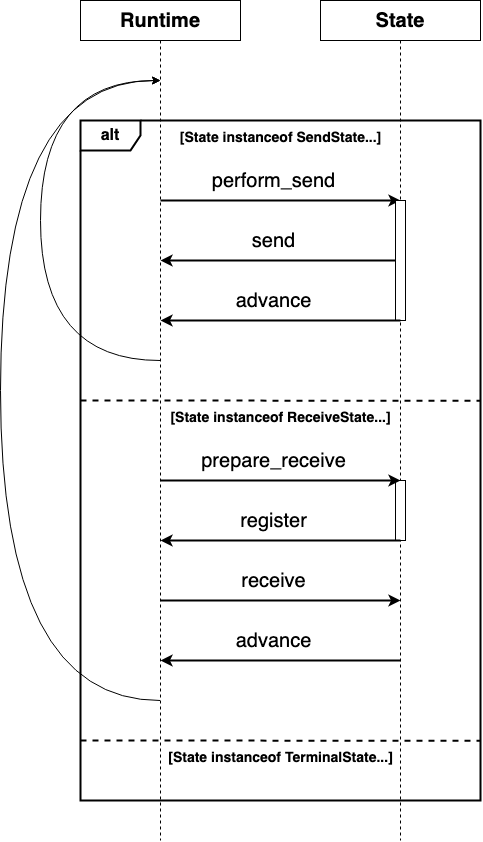
\includegraphics[width=0.5\textwidth]{NodeRuntimeEFSM}
\captionof{figure}{``Message Passing'' Abstraction of EFSM Execution for
Server Endpoints}
\label{fig:noderuntimeefsm}
\end{figure}

\subsection{Sending Messages}
\label{subsection:noderuntimesend}

This is rather straightforward: 
we show the generated code in \cref{lst:nodesend}.

\begin{figure}[!h]
\begin{lstlisting}[language=javascript,tabsize=2]
export class S54 extends ISend {
	constructor(private handler: Handler.S54) { super(); }

	performSend(
		next: EfsmTransitionHandler,
		send: (role: Roles.Peers, label: string, payload: any[]) 
			=> void
	) {
		const [label, payload, successor] = this.handler;
		send(Roles.Peers.Client, label, payload); (*@\label{line:nodesendrole}@*)
		return next(successor);
	}
}
\end{lstlisting}
\captionof{lstlisting}{Generated Code for \texttt{Implementation} API for
Send State}
\label{lst:nodesend}
\end{figure}

We get the label, payload and successor implementation
directly from the handler implemented by the developer, 
accurately typed by how we define the handler API in \filename{EFSM.ts}.
The developer does not need to specify which role
to send to: this is a sensible design choice, as we know this
from the Scribble protocol, so we do not need the developer 
to specify separately.
As a result, we generate the code to send the message
to the correct role (\cref{line:nodesendrole}).
We use the \texttt{send()} method passed down
by the runtime to commit our communication action:
the runtime will handle how to serialise the message and perform
the send. We guarantee that \texttt{send()} is called
\textbf{exactly once} by construction, thus channel linearity
is never violated.
Finally, we use the parameterised EFSM transition handler
to notify the runtime which specific state to transition to.

\subparagraph{Sending through WebSockets}
We define message structures as interfaces, which
are represented by objects. 
By convention in \fancyname{SessionTS},
we serialise messages into \textit{JavaScript Object Notation}
(or JSON) \cite{json} using the built-in \texttt{JSON.stringify()}
method.

\begin{lstlisting}[language=javascript]
send(role: Roles.Peers, label: string, payload: any[]) {
	this.roleToSocket[role].send(JSON.stringify({
		label, payload
	});
}
\end{lstlisting}

They are decoded using the same interface schema on the receiving end
using \texttt{JSON.parse()}.
Whilst the method return type is the
dynamic \lstonelinejs{any} type, 
we guarantee type safety by construction
as we performed the serialisation in the first place, so
we can safely interpret the deserialised content 
using a concrete type.

\subsection{Receiving Messages}
\label{subsection:noderuntimereceive}

We need to update the message event listener on the WebSocket
to use the developer's handler -- 
specific to the \textit{current state} -- 
to process the message.
Our approach is to keep the WebSocket message event listener
untouched, but define it in a way that allows \textit{dynamic} behaviour.
We walk through the concept implemented in (\cref{lst:noderuntimewsmsg}):

\begin{enumerate}
\item 
\texttt{Session} keeps track of the \textit{current}
message receive handler (\cref{line:noderuntimehandler}).
The \texttt{?} syntax denotes it is an \textit{optional}
type: not every state is a receive state, so there does not \textit{have} to
be an active message handler.

\item
The receive handler does \textit{not} need a specialised type
(\cref{line:msghandler}). The receive handler is defined in
the \texttt{Implementation} class of the concrete receive state,
so it will deserialise the message to the correct form.

\item
The \texttt{register()} method (\cref{line:register})
is passed to the \texttt{Implementation} class of the concrete
receive state, which will construct the message handler
around the developer's handler implementation and register it
with the runtime.

\item
When a message is received from the channel,
we dynamically process it with 
the current registered handler (\cref{line:callhandler}).
We encapsulate this dynamic behaviour in an instance method
and bind it as an event listener (\cref{line:wsbind})
for the WebSocket connection
of each non-server endpoint.
\end{enumerate}

\begin{figure}[!h]
\begin{lstlisting}[language=javascript,tabsize=2]
type MessageHandler = (message: any) => void; (*@\label{line:msghandler}@*)

class Session {
	// Optional type, same as `MessageHandler | undefined`
	private handler?: MessageHandler; (*@\label{line:noderuntimehandler}@*)

	constructor(...) {
		...
		// Process incoming messages from each WebSocket
		// using `this.receive()`
		Object.values(this.roleToSocket).
			.forEach(ws => ws.onmessage = this.receive.bind(this)); (*@\label{line:wsbind}@*)
			
		// Initialise handler as undefined
		this.handler = undefined;
	}
	
	// Set the handler to be used to handle the next receive event
	register(handler: MessageHandler) { this.handler = handler; } (*@\label{line:register}@*)

	receive({ data }: WebSocketMessage) {
		const handler = this.handler; (*@\label{line:callhandlerstart}@*)
		
		// `Unregister` the current receive handler
		this.handler = undefined; (*@\label{line:callhandler2}@*)
		
		// `handler` has an optional type, so we first
		// check if there is a value set, then invoke the handler.
		// Same as `if (handler !== undefined) { handler(data); }`
		handler?.(data); (*@\label{line:callhandler}@*)
	}
}
\end{lstlisting}
\captionof{lstlisting}{Attempt to Dynamic WebSocket Message Event Listener}
\label{lst:noderuntimewsmsg}
\end{figure}

We also show the generated code for the \texttt{Implementation}
class of the receive state in \cref{lst:nodereceive}
-- this should appear consistent
with the explanation above.

\begin{figure}[!h]
\begin{lstlisting}[language=javascript,tabsize=2]
export class S51 extends IReceive {
	
	constructor(private handler: Handler.S51) { super(); }

	prepareReceive(
		next: EfsmTransitionHandler,
		register: (from: Roles.Peers, messageHandler: MessageHandler)
			=> void
	) {
		// Define dynamic WebSocket message event listener
		const messageHandler = (message: any) => {
		
			// Deserialise message
			const decoded = JSON.parse(message) as Message.S51;
			
			// Discriminate between messages using label
			switch (decoded.label) {
				case Labels.S51.ADD: {
					// Invoke handler to get successor state
					const successor = 
						this.handler[decoded.label](...decoded.payload);
						
					// Invoke callback to advance EFSM
					return next(successor);
				}
				case Labels.S51.QUIT: {
					const successor = 
						this.handler[decoded.label](...decoded.payload);
					return next(successor);	
				}
			}            
		}
		
		// Register the message handler under the
		// WebSocket bound to the `Client` role
		register(Roles.Peers.Client, messageHandler);
	}
}
\end{lstlisting}
\captionof{lstlisting}{Generated Code for \texttt{Implementation} API for
Receive State}
\label{lst:nodereceive}
\end{figure}

Ideally, a more succinct (and direct) representation would be
\begin{lstlisting}[language=javascript]
(message: any) => {
	const decoded = JSON.parse(message) as Message.S51;
	const successor = 
		this.handler[decoded.label](...decoded.payload);
	return next(successor);
}
\end{lstlisting}

But this expresses a type dependency between \texttt{label}
and \texttt{payload} which, as discussed 
(\cref{subsubsection:dependenttypes}), cannot be implemented.
However message structures \textit{precisely} 
define a discriminated union 
(the label acts as the discriminant 
to distinguish between payload types),
so we handle this with a switch statement,
at the cost of having the same code in each case --
TypeScript does infer the correct specific type in each case statement,
so code duplication here does serve a functional purpose.

Returning to \cref{lst:noderuntimewsmsg},
note that the type of the \texttt{handler} property is \textit{optional}
-- this hints at a problem: 
\textit{how do we know that \texttt{this.handler} is set when
a message is received?} The types imply that we \textit{do not},
and this is indeed the case.
In fact, when we consider a \textit{multiparty} context,
our approach with receive handler registration 
using an optional value actually \textit{fails} to guarantee correctness.
We motivate the problem with a worked
example.

\begin{example}[``Out-of-order'' message receives]
Recall that Node.js is a single-threaded event loop runtime, so
when a message arrives, 
the \texttt{onmessage} event is \textit{queued},
and current execution is \textit{not pre-empted}.

Now consider a multiparty session specified by the global type

\[
A \to S: \text{\lstonelinejs{M1(string)}}.~ 
B \to S: \text{\lstonelinejs{M2(number)}}.~\texttt{end} 
\]

Suppose \trole{S} is the server endpoint.
We describe a possible execution flow for the protocol
that breaks our implementation:

\begin{enumerate}
\item 
\trole{S} transitions to its initial state, 
``receive \lstonelinejs{M1(string)} from \trole{A}''.
The receive handler for \tmsg{M1} is registered.

\item
\tmsg{M2} arrives at \trole{S}, so the \texttt{onmessage} handler
is queued. This is \textit{perfectly plausible}: there
is no causal relation between \tmsg{M1} and \tmsg{M2}.

\item
\tmsg{M1} arrives at \trole{S}, so the \texttt{onmessage} handler
is queued.

\item
The \texttt{onmessage} handler for \tmsg{M2} is executed.
The registered handler expects \lstonelinejs{M1(string)},
but it is called with \lstonelinejs{M2(number)}, which raises
a runtime type error.
\end{enumerate}

This exposes a problem: 
the order of message \textit{arrivals} may not
correspond with the order of \textit{receiving} messages as
specified in the protocol,
\textit{so} the message may arrive before its
corresponding handler is registered.
\end{example}

We observe that message arrivals do not have to be causally related.
However, if we consider a similar \textit{binary} example
\[
A \to S: \text{\lstonelinejs{M1(string)}}.~ 
A \to S: \text{\lstonelinejs{M2(number)}}.~\texttt{end}
\]
then \tmsg{M1} \textit{must} arrive before \textit{M2},
since this is sent through the WebSocket connection between 
\trole{A} and \trole{S}, and FIFO guarantees are respected 
for each individual WebSocket connection. 
We visualise the possible orders of message receive events
in \cref{fig:nodereceivecompare}.

\begin{figure}[!h]
\centering
\begin{subfigure}[b]{0.8\textwidth}
\centering
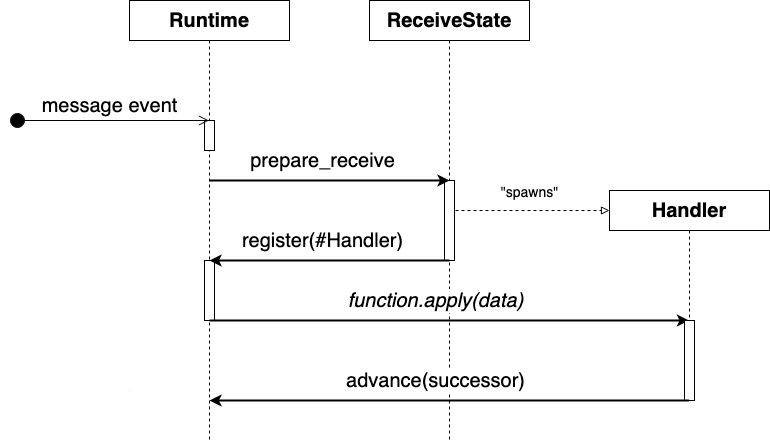
\includegraphics[width=\textwidth]{NodeRuntimeReceive2}
\caption{Message processed before transitioning to receive state}
\label{subfig:nodereceivemsgfirst}
\end{subfigure}
\hfill
\begin{subfigure}[b]{0.8\textwidth}
\centering
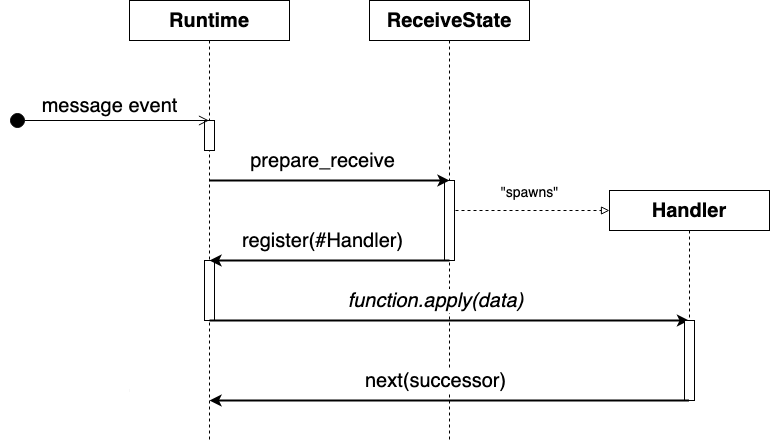
\includegraphics[width=\textwidth]{NodeRuntimeReceive1}
\caption{Message processed after transitioning to receive state}
\label{subfig:nodereceivehandlefirst}
\end{subfigure}
\caption{Possible Orderings for Receiving Message and
Registering Handler}
\label{fig:nodereceivecompare}
\end{figure}

We observe that defining the handler using an optional type
is insufficient. We need a similar mechanism for handling messages
waiting for handlers, and we cannot assume an ordering on the arrival
of messages that are not causally related.

We proceed to generalise our approach from one optional-type
handler to two mappings:
\textbf{(1)} a mapping from endpoint to message queues\footnote{
TypeScript arrays have built-in $O(1)$ time complexity
\texttt{shift()} and \texttt{push()} operations, which
can be used as a queue.}, and
\textbf{(2)} a mapping from endpoint to handler queues.
To simply put, if an incoming message is waiting for its handler,
it gets enqueued in the message queue labelled by the sender of the message;
when the handler is created, it pops the message off the queue 
and directly processes it; the same logic applies for a handler waiting
for its message.
We could have used a mapping from endpoint to optional type,
but queue operations elegantly hides the mechanics of
\cref{line:callhandlerstart,line:callhandler2,line:callhandler}
in \cref{lst:noderuntimewsmsg}.

We outline the changes made to the \texttt{Session} class,
as shown in \cref{lst:nodesession}:

\begin{enumerate}
\item We construct types for these two mappings 
(\cref{line:mapped1,,line:mapped2}), 
using a generic mapped typed defined below.
\begin{lstlisting}[language=javascript]
// Inside the Roles namespace...
export type PeersToMapped<Value> = { [Role in Peers]: Value };
\end{lstlisting}

\item Empty queues are initialised for both mappings
(\cref{line:queue1,,line:queue2}).

\item Each endpoint has a different \texttt{onmessage}
event listener, which will interact with the message queue
and handler queue corresponding to that endpoint. 
We achieve this by changing the \texttt{receive()} method
to be parameterised on the role instead 
(\cref{line:receivefunc}),
so it \textit{generates} an event listener 
(\cref{line:receivefuncret})
tailored for receiving messages
from that particular role.

\item
The \texttt{register()} method now also takes the role
as a parameter (\cref{line:newregister}) in order to check the 
corresponding pair of queues.
\end{enumerate}

\begin{figure}[!h]
\begin{lstlisting}[language=javascript,tabsize=2]
type RoleToMessageQueue = Roles.PeersToMapped<any[]>; (*@\label{line:mapped1}@*)
type RoleToHandlerQueue = Roles.PeersToMapped<MessageHandler[]>; (*@\label{line:mapped2}@*)
type RoleToSocket = Roles.PeersToMapped<WebSocket>;

class Session {
	...
	private roleToSocket: RoleToSocket;
	private messageQueue: RoleToMessageQueue;
	private handlerQueue: RoleToHandlerQueue;
	
	constructor(...) {
		...
		Object.values(Roles.Peers).forEach(role => {
			const socket = this.roleToSocket[role];
			socket.onmessage = this.receive(role).bind(this);
		});
		
		// Set up empty queues
		this.messageQueue = { [Roles.Peers.Client]: [], }; (*@\label{line:queue1}@*)
		this.handlerQueue = { [Roles.Peers.Client]: [], }; (*@\label{line:queue2}@*)
		
		this.next(initialState);		// Advance to initial state
	}
	
	receive(from: Roles) { (*@\label{line:receivefunc}@*)
	
		// Return a WebSocket message event listener
		// that looks at the message/handler queue
		// specific to the `from` role
		
		return ({ data }) => { (*@\label{line:receivefuncret}@*)
			// Array.shift() can return undefined if empty
			const handler = this.handlerQueue[from].shift();
			if (handler !== undefined) {
				handler(data);
			} else {
				this.messageQueue[from].push(data);			
			}
		}
	}
	
	register(from: Roles.Peers, handler: MessageHandler) { (*@\label{line:newregister}@*)
		const message = this.messageQueue[from].shift();
		if (message !== undefined) {
			handler(message);		
		} else {
			this.handlerQueue[from].push(data);		
		}
	}
}
\end{lstlisting}
\captionof{lstlisting}{Modified \texttt{Session} class to correctly
handle message receive events}
\label{lst:nodesession}
\end{figure}

Each endpoint must have consistency between
its message queue and handler queue.
We get the consistency from the simple fact that Node.js 
is a single-threaded runtime and execution is never pre-empted,
so there is no need to worry about atomic queue operations or
locking data structures.

We walk through how this design addresses the problems
in the previous example.

\begin{example}[Revisiting ``out-of-order'' message receives]
Consider the same multiparty session specified by the global type

\[
A \to S: \text{\lstonelinejs{M1(string)}}. 
B \to S: \text{\lstonelinejs{M2(number)}}. \texttt{end} 
\]

We show that our modified implementation addresses the problem:

\begin{enumerate}
\item 
\trole{S} transitions to its initial state,
``receive \lstonelinejs{M1(string)} from \trole{A}''.
\textit{The message queue for \trole{A} is empty,}
so the receive handler for \tmsg{M1} is registered 
\textit{under the handler queue for \trole{A}.}

\item
\tmsg{M2} arrives at \trole{S}, so the \texttt{onmessage}
handler is queued.

\item
\tmsg{M1} arrives at \trole{S}, so the \texttt{onmessage} handler
is queued.

\item
The \texttt{onmessage} handler for \tmsg{M2} is executed.
\textit{The handler queue for \trole{B} is empty, 
so \tmsg{M2} is added to the message queue for \trole{B}}.

\item
The \texttt{onmessage} handler for \tmsg{M1} is executed.
\textit{The handler queue for \trole{A} is non-empty,
so the handler is popped off the front of the queue 
and processes \tmsg{M1}.}

\item
\trole{S} transitions to the successor state, 
``receive \lstonelinejs{M2(number)} from \trole{B}''.
\textit{The message for \trole{B} is non-empty,
so \tmsg{M2} is popped off the queue and 
processed by the handler.}
\end{enumerate}

This execution is free of communication mismatches.
\end{example}

\subsection{Handling Termination}
WebSocket connections should be closed when the session terminates,
and both the browser endpoint and the server endpoint are capable
of closing connection. As we generate code for both, we define
a convention that the browser endpoint will close 
the WebSocket connection,
so we do nothing for this state at \cref{lst:noderuntime}.
\section{Alternative Designs}
\begin{itemize}
\item not sure whether to put this in the subsection above so it flows better?
\item naive implementation is to pass the send() function as a prop for the developer to incorporate in their event listener -- this is most flexible, but we cannot provide static guarantees
\item factory approach -- the runtime could pass a factory function which, takes an UI element and performs the binding; this is better, as channel resources are not exposed, but the adversarial-minded developer can later override the event listener in the DOM etc
\end{itemize}
\section{Limitations}
\label{section:nodelimitations}

Providing \textbf{static} communication safety guarantees have
come at a cost of providing relatively verbose APIs to the developer,
which introduces a learning curve. In particular,
the distinction between the \texttt{Implementation} and
\texttt{Handler} API should be an internal detail, but
the developer still needs to use the \texttt{Implementation} API
in their logic. 

Our APIs also rely on state identifiers, which also
does not help code readability, as it is neither apparent nor
self-documenting what \texttt{S51} refers to -- some existing work
\cite{Hybrid2016} augment the state identifiers with the channel
action and labels involved (e.g. 
\texttt{S51_Receive__Add_Number__Quit_String}).

Using handler-style APIs also mean that we require
nested scoping to propagate values between states,
which does not scale elegantly as the levels of nesting
increase. For example, the following implementation of
the \tprotocol{One Adder} protocol would be invalid if
we define the handlers for the continuations separately,
because the received payload are no longer in scope
(\cref{line:notinscope}).

\begin{lstlisting}[language=javascript]
const first = new S4({ NUM1: (x) => secondOperand, });
const second = new S6({ NUM2: (y) => sum, });
const sum = [Labels.S7.SUM, (*@\label{line:notinscope}\hl{???}@*), new S5()];
\end{lstlisting}

However, the developer may choose to propagate values
between states through persistent storage APIs (such as
storing values in a database and retrieving them for
handlers of continuation states), so our generated APIs
do not strictly enforce scoping to be the only way to
propagate values in the application logic.

%\section{Summary}
%\begin{itemize}
%\item static guarantees on avoiding communication mismatch
%\item static guarantees on affine channel usage
%\item leverage the react framework to express the model types approach from Fowler 2020 appropriately, to provide static guarantees, by construction, that the channel actions made available at each state respect the protocol, and by definition, multiparty session type safety
%\end{itemize}